\chapter{Survey Application}
\textbf{TEXTTTTTTTT}
\section{Application of X-BAP}

In this section, the methodology of applying \gls{x-bap} to \gls{mer} mosaics is explained. To apply the \gls{x-bap} method to images from \gls{edf}, several inputs are required: observations, coordinates of sources, \glspl{psf}, and the \gls{rms} map.

\subsection{PSF}

The MER catalog has a \gls{psf} grid. This can be used to find a more accurate \gls{psf} for each part of the image by interpolating between grid points. However, in \gls{x-bap} this is computationally expensive as the prefactor in \autoref{eq: numerical deconvolution} then needs to be recalculated for every single source. Instead of that approach, the \glspl{psf} in the grid are averaged to obtain a single \gls{psf} that represents the seeing across the entire image, which is used for the aperture flux.

% \subsection{PSF Construction}

% The PSFs of the Rubin images are readily available, but the PSFs of the Euclid images are not. So those need to be created before pca-phot can be applied to its images.

% For this, the Source EXtractor \citep{1996A&AS..117..393B} is used to find the fluxes and full-width half-maxima (FWHM) of different sources in the image. Taking the natural logarithm of both sides and plotting the results yields the image shown in \autoref{fig: Chimney}. 

% \begin{figure}[H]
%     \centering
%     \includegraphics[width=0.3\linewidth]{placeholder.pdf}
%     \caption{The flux of the sources in the VIS-band for different FWHM. The vertical strip of sources is saturated stars in the image. These stars can be used to create an estimate of the PSF. }
%     \label{fig: Chimney}
% \end{figure}
% The stretch of sources that form a vertical line are the saturated stars, which are point sources.  This means that after convolution with the PSF, they have the same shape as the PSF. These sources can be stacked to create an estimate for the PSF in that image. 


\subsection{Noise Square}

Find a square with the minimal variance. This square should contain no sources, so it should be only background noise. This noise square is used to calculate the correlation between the pixels for the MER mosaics (following \Cref{subsec: Noise from RMS}).

\textbf{EXPLAIN HOW THIS IS FOUND + image}



% \subsection{Fitting Weights}

% To find the pre-seeing weight function, a Gaussian is fitted to the objects in the image. This is done in the VIS as this band has the highest resolution and quality. Next, Gaussian-shaped galaxies with different scales are simulated and convolved with the different \gls{psf} of all the filters in \autoref{tab:mer filters}. \gls{x-bap} is applied to the images using differently sized pre-seeing weight functions, which gives the \gls{snr} over the different sizes of weight functions. These curves are normalized by dividing by the maximum and then added together to get a single curve that represents the \gls{snr} across all filters. The maximum of this curve is linked to the size of the Gaussian in the pre-seeing image. This gives a relation between the pre-seeing image size and the optimal pre-seeing weight function size to maximize the \gls{snr} across the different filters. A 6th-order polynomial is fitted to this relation. 

% Now that there is a semi-empirical relation between the size of the source and the optimal weight size, a Gaussian is fitted to the sources in the VIS band. Following this, the pre-seeing size is estimated by using the size of the \gls{psf} of the VIS band $\sigma_\mathrm{fit}^2\approx\sigma_\mathrm{intrinsic}^2+\sigma_\mathrm{VIS-PSF}^2$. The intrinsic size is then converted to a weight function size by using the polynomial.

\subsection{Applying X-BAP Algorithm}\label{subsec: applying pca-phot algorithm}
The coordinates and \gls{fwhm} from the \gls{mer} catalogs are used to find the flux of sources in the \gls{mer} tiles.
For each source, a cutout is made around it to determine the flux in that region. The cutout is 128 pixels for the \gls{mer} mosaic, which corresponds to a physical size of 12.8". However, the center of the sources is not necessarily exactly the center of the cutout due to the discrete number of pixels in the image. 
Defining the fractional coordinates as
\begin{equation}
    dx = x - \lfloor x\rfloor,\;dy = y - \lfloor y\rfloor.
\end{equation}

The weight function has to be shifted to the correct sub-pixel position. This can be done by multiplying the Fourier transform of the weight function by a phase factor that depends on the shift of the weight function. By modifying \autoref{eq: numerical deconvolution}, the new weight function becomes
\begin{equation}\label{eq: numerical deconvolution v2}
    W^i_\mathrm{A} = \mathcal{F}^{-1}\left\{\frac{\mathcal{F}\{\bar{P}_i\}^*}{|\mathcal{F}\{\bar{P}_i\}|^2+K}\cdot\mathcal{F}\{\tilde{W}_\mathrm{A}\}\cdot\exp(-2\pi i(k_xdx+k_ydy))\right\}.
\end{equation}
This allows for the reuse of the same-sized weight function for different sources. The sizes of the pre-seeing weight functions are 0.5, 1, and 2 times the \gls{fwhm} given by the \gls{mer} catalogs, following a similar procedure as \cite{euclid_collaboration_euclid_2026}. The \gls{fwhm} are determined from the worst filter and are therefore a good way to find what size of weight function can be used, as the weight function needs to be larger than the \gls{psf} of the worst band. Furthermore, 0.5\gls{fwhm} can be used as the scale parameter for the weight function, as the \gls{fwhm} of a Gaussian is $\mathrm{FWHM}=2\sqrt{2\ln2}\sigma\approx2.355\sigma$. This means that $0.5\mathrm{FWHM}>\sigma$. This ensures that the size of the aperture is larger than the largest \gls{psf}.

\newpage
\section{Source Classification}

The colors calculated using the different sizes of the weight functions give information about the properties of the observed sources in the Euclid fields. Furthermore, the size of a source in the sky also gives information on the type of the object; stars and \glspl{qso} are point sources, while galaxies are generally extended.


\subsection{Splitting Based on Colors}\label{subsec: splitting based on colors}
To separate sources into groups of sources that have similar colors to either stars or galaxies, \gls{umap} is used. \textbf{EXPLANATION OF UMAP + PARAMS USED}. After the dimension reduction of the color data, DBSCAN \citep{ester_density-based_1996} is used to label the sources into two groups: one with sources that have star-like colors, and one with sources that have galaxy-like colors.

\subsection{Differentiating between Point-Sources and Extended Sources}

As \gls{x-bap} is a way to apply a weight function on the pre-seeing image, point sources can be represented by delta functions in this pre-seeing image. The weight functions are centered on the objects, which means that for point sources, the flux is completely independent of the size of the weight function, as the value of the weight function at the center is constant for different sizes of the weight functions. However, for extended sources, increasing the size of the pre-seeing weight function increases the flux. This can be used to divide the sources into a group of point sources and a group of extended sources.

\begin{figure}[H]
    \centering
    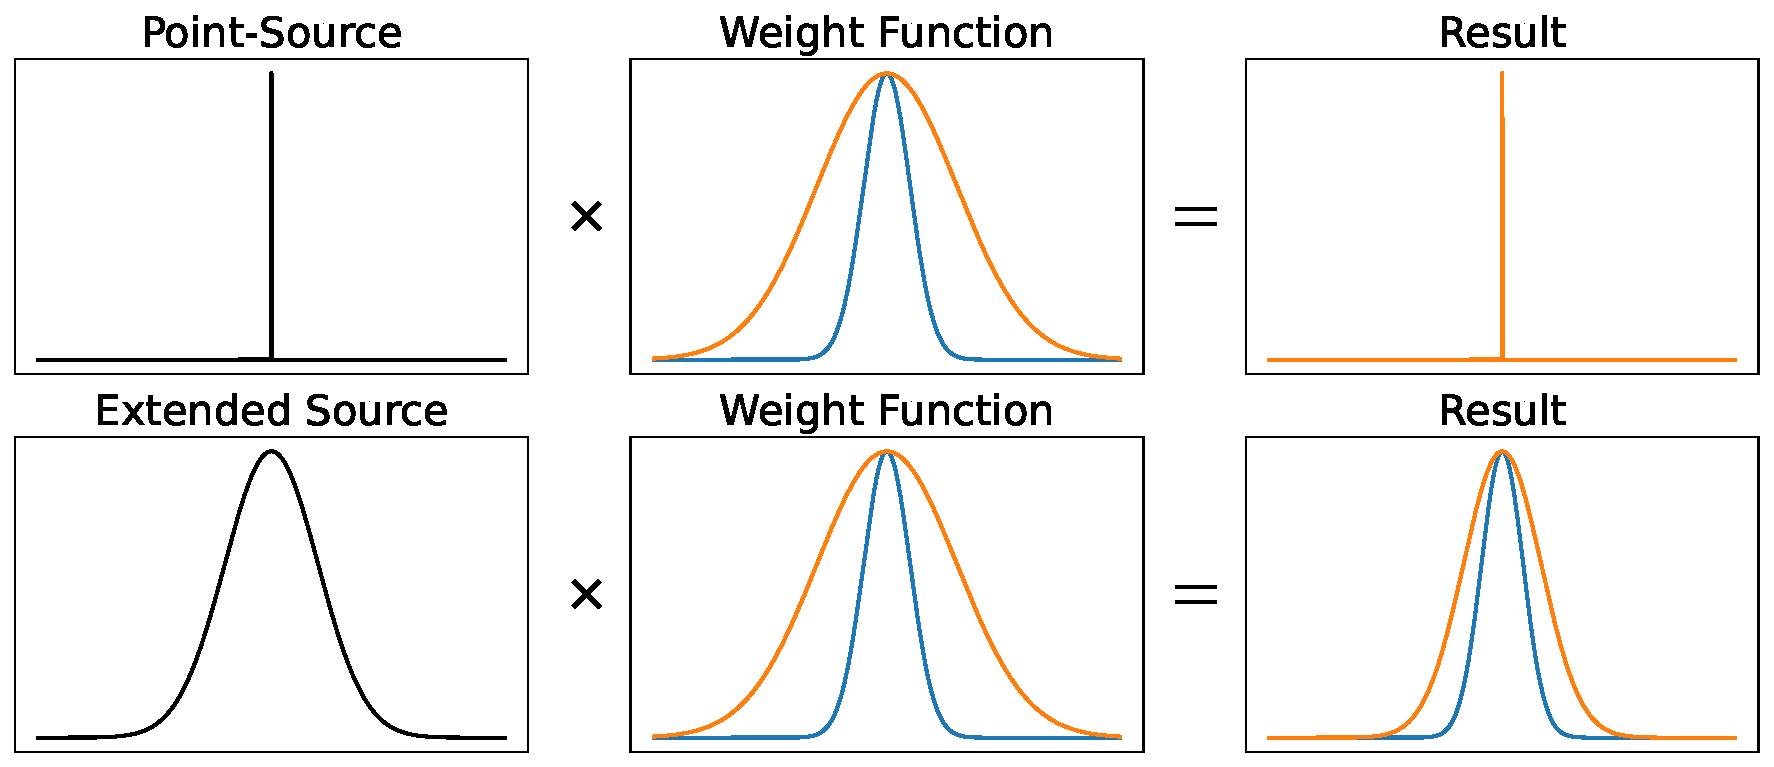
\includegraphics[width=0.9\linewidth]{results/figures/analysis/point_vs_extended.pdf}
    \caption{The difference in the aperture flux for a point source and an extended source. When a Gaussian weight function is centered on the source, the aperture flux is the same for different sizes of the weight function, but for an extended source the aperture flux increases when the size of the weight function increases.}
    \label{fig:placeholder}
\end{figure}
This means that the difference in flux for different-sized weight functions gives information about the physical size of the source in the image. A similar procedure is followed as in \autoref{subsec: splitting based on colors}, except the fractional difference between different weight sizes in each band is added into the parameters that \gls{umap} reduces the dimensionality of. Those are defined as
\begin{align}
\Delta_{\mathrm{1,i}} &= \frac{F_{\mathrm{1FWHM,i}}-F_{\mathrm{0.5FWHM,i}}}{F_{\mathrm{1FWHM,i}}}, \\
\Delta_{\mathrm{2,i}} &= \frac{F_{\mathrm{2FWHM,i}}-F_{\mathrm{1FWHM,i}}}{F_{\mathrm{2FWHM,i}}}, \\
\Delta_{\mathrm{3,i}} &= \frac{F_{\mathrm{2FWHM,i}}-F_{\mathrm{0.5FWHM,i}}}{F_{\mathrm{2FWHM,i}}},
\end{align}
where i denotes the band in which the flux is computed. These are the fractional changes in the flux for the different weight functions. The choice of division is always to divide by the flux from the larger weight function of which the difference is calculated. This is because the large weight function should give a more stable result. Using these parameters in combination with the colors should help to distinguish sources that are extended and those that are not.
The results of this are compared to the results from \cite{euclid_collaboration_euclid_2026}, which used the colors to classify sources into stars, galaxies, and \glspl{qso}.



% \section{Photometric Redshift Estimation}
% Eazy \citep{brammer_eazy_2008}
\newpage
\section{Application Results}

In this section, the application of the \gls{x-bap} method on the \gls{mer} mosaics is discussed, including the preprocessing. The results are compared to the colors derived from the flux measurements in the \gls{mer} catalogs. 

% \subsection{Preprocessing}
% \textbf{ZEROPOINT}
% The \glspl{psf} of tile \textbf{TILEINDEX} is used to determine the relationship between the source size in the VIS band and the weight-function size that optimizes the \gls{snr} of the flux across all bands. A Gaussian object is simulated with Gaussian noise. Different sizes of weight functions are used to find the \gls{snr} for each of the \glspl{psf}. For each of the \glspl{psf}, the curve is divided by its maximum, and the results are summed to obtain a single curve that captures the combined \gls{snr} across all the \glspl{psf}. The size of the weight function where this curve is maximized is combined with the size of the source. This is repeated for different sizes of the source, resulting in a relation between the size of the source and the size of the weight function that maximizes the \gls{snr}. A 5th-order polynomial is fitted to the measurements. 
% \begin{figure}[H]
%     \centering
%     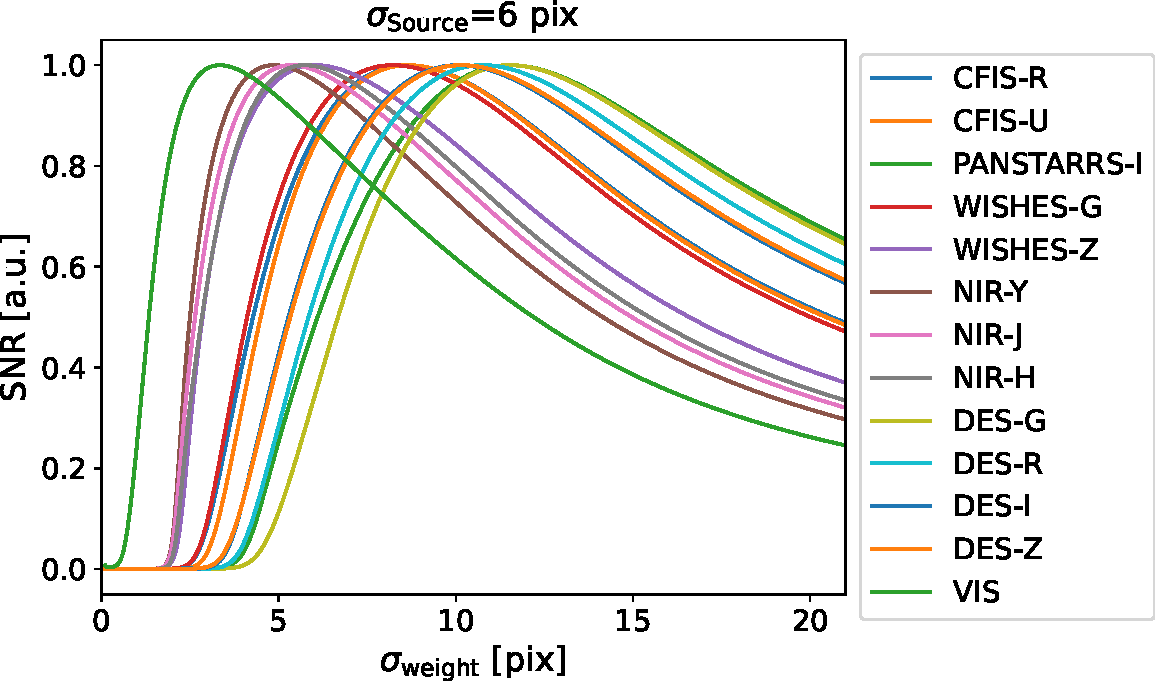
\includegraphics[width=0.5\linewidth]{results/figures/observation/weight_snr.pdf}
%     \caption{The relation between the size of the Gaussian weight function that maximizes some form of the \gls{snr} over all bands compared to the size of the source in the VIS field. }
%     \label{fig: weight snr}
% \end{figure}
% \begin{figure}[H]
%     \centering
%     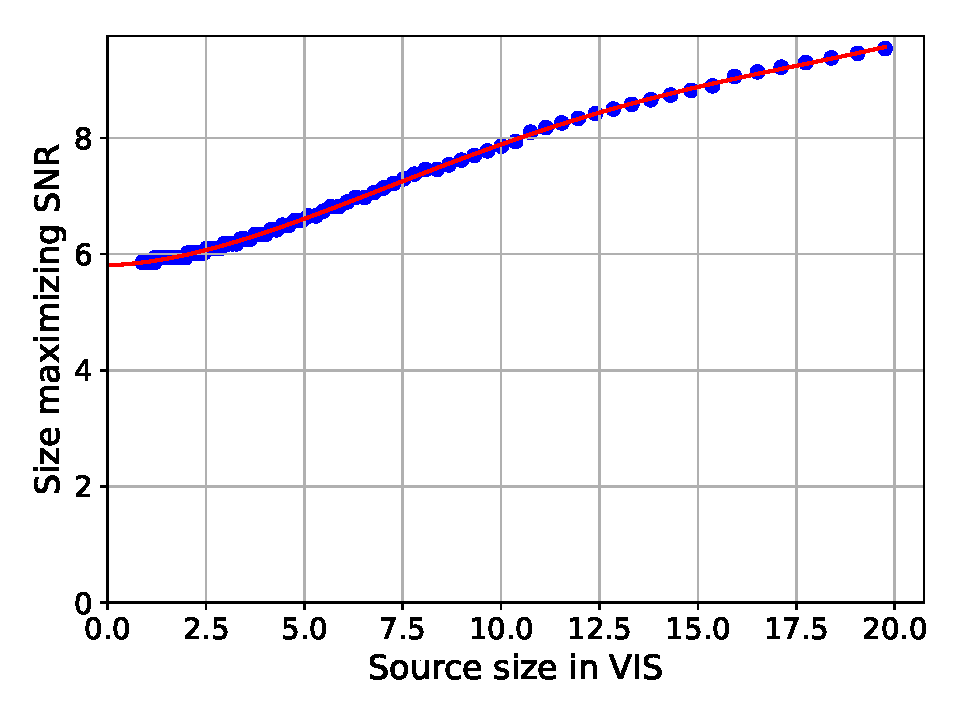
\includegraphics[width=0.5\linewidth]{results/figures/observation/best_weight_snr.pdf}
%     \caption{The relation between the size of the Gaussian weight function that maximizes some form of the \gls{snr} over all bands compared to the size of the source in the VIS field. }
%     \label{fig: best weight snr}
% \end{figure}

% \begin{table}[H]
% \centering
% \begin{tabular}{l c}
% \hline
% \textbf{Survey / Band} & \textbf{PSF Scale (arcsec)} \\
% \hline
% CFIS-R      & 0.36 \\
% CFIS-U      & 0.38 \\
% PANSTARRS-I & 0.52 \\
% WISHES-G    & 0.35 \\
% WISHES-Z    & 0.23 \\
% NIR-Y       & 0.20 \\
% NIR-J       & 0.22 \\
% NIR-H       & 0.23 \\
% DES-G       & 0.58 \\
% DES-R       & 0.50 \\
% DES-I       & 0.45 \\
% DES-Z       & 0.46 \\
% VIS         & 0.09 \\
% \hline
% \end{tabular}
% \caption{\gls{psf} scale parameters for different surveys and bands.}
% \label{tab:psf_scales}
% \end{table}


% Next, a Gaussian is fitted to the sources in the \gls{mer} tiles, which is used to find the best weight size to optimize the \gls{snr}. The coordinates in the \gls{mer} catalog are used to set the centers of the objects, which will also be used for the flux measurements. The distribution of the fitted sizes of the sources is shown in \textbf{LINK FIGURE}.

% \textbf{FIGURE WITH THE DISTRIBUTION OF THE SIZES OF THE OBJECTS IN THE IMAGES}

% The sizes of the weight function are clipped between 0.7" and 1.2". The lower bound is to make sure that the weight function is bigger than the largest \gls{psf}. The upper bound is to prevent the fringing effect of the deconvolution. 


\subsection{Multi-Band Flux Measurements}
Using the \gls{fwhm} of the \gls{mer} catalog, fluxes for objects in the \gls{mer} tiles are calculated, and measurement errors are estimated from the \gls{rms} maps. A selection of the sources is made based on the \gls{snr}, considering only sources that have an \gls{snr} greater than 5 in each of the bands considered. 

\begin{figure}[H]
    \centering
    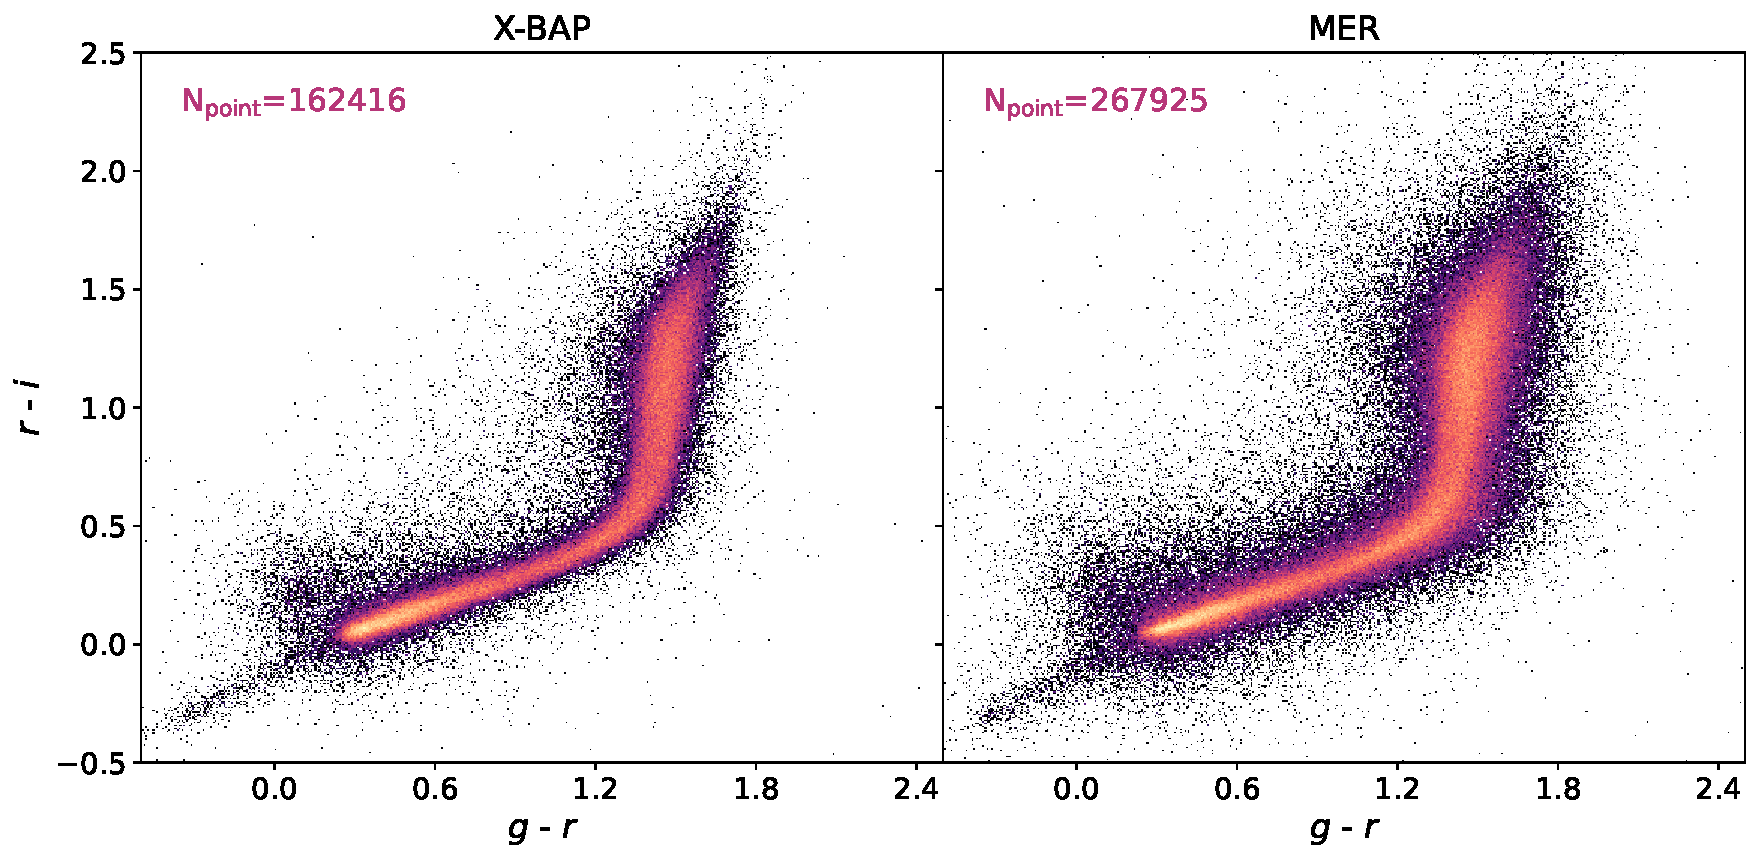
\includegraphics[width=0.9\linewidth]{results/figures/analysis/GRRI_gaap_catalog_cutoff_5.pdf}
    \caption{Color-color diagram of the point-like sources. The colors are derived from the flux in the \gls{des} filters g, r, and i. The sources in the image are those with a point-source probability $\geq$70\% given by the \gls{mer} catalog.}
    \label{fig:color color gri}
\end{figure}
The flux measurements of the point sources in the \gls{edf} show that the number of sources that have an \gls{snr} greater than 5 in the \gls{mer} catalog is larger than that of the \gls{x-bap}. In both cases, the distribution is narrower towards the blue (bottom left) than towards the redder end (top right). Furthermore, there is a streak of objects that are much bluer than most other objects. These are most likely \glspl{qso}. The position of the point sources in the color-color diagram is nearly identical between the \gls{x-bap} method and the \gls{mer} catalogs. 


\begin{figure}[H]
    \centering
    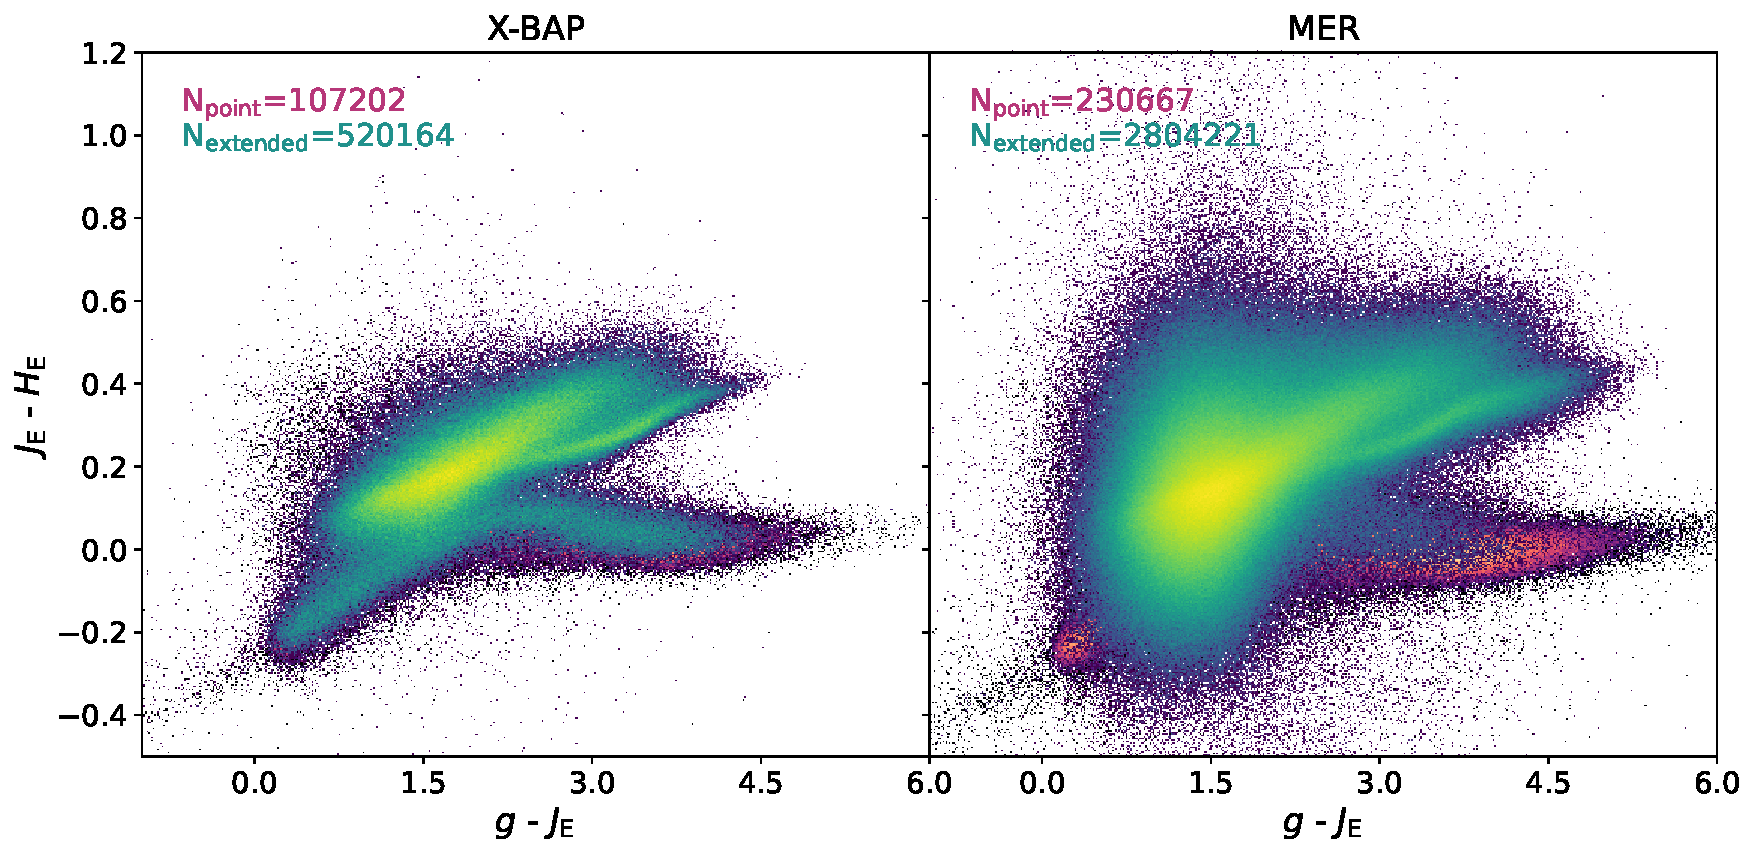
\includegraphics[width=0.9\linewidth]{results/figures/analysis/GJJH_gaap_catalog_cutoff_5.pdf}
    \caption{Color-color diagram of point-like and extended sources. The colors are derived from the flux in the \gls{des} filter g, and the \gls{nisp} filters J$_E$ and H$_E$. The point-like sources in the image are the objects in the \gls{mer} catalog with a point-source probability $\geq$70\% given by the \gls{mer} catalog, and the extended sources are those with a point-source probability <70\%.}
    \label{fig:color color gHHJ}
\end{figure}
\autoref{fig:color color gHHJ} shows that the number of sources in the selection of \gls{mer} sources is larger than that of the \gls{x-bap}, just like in \autoref{fig:color color gri}. There appear to be 2 large distributions of sources. A group that is concentrated towards the bottom. These are largely objects that have a point-source probability $\geq$70\%. However, there is also contamination of sources that have a lower point-source probability. In the upper group of sources, there is a smaller group of sources that branches from the main population of sources with a point-source probability <70\%. The different number of sources in both selection suggest one of three options: (i) \gls{x-bap} is less accurate than the method used to calculate the flux in the \gls{mer} catalogs, (ii) \gls{x-bap} overestimates the noise on the flux, which decreases the number of sources in the selection, or (iii) the method used to calculate the flux in the \gls{mer} catalogs underestimates the noise on the flux, which increases the number of sources in the selection.

\begin{figure}[H]
    \centering
    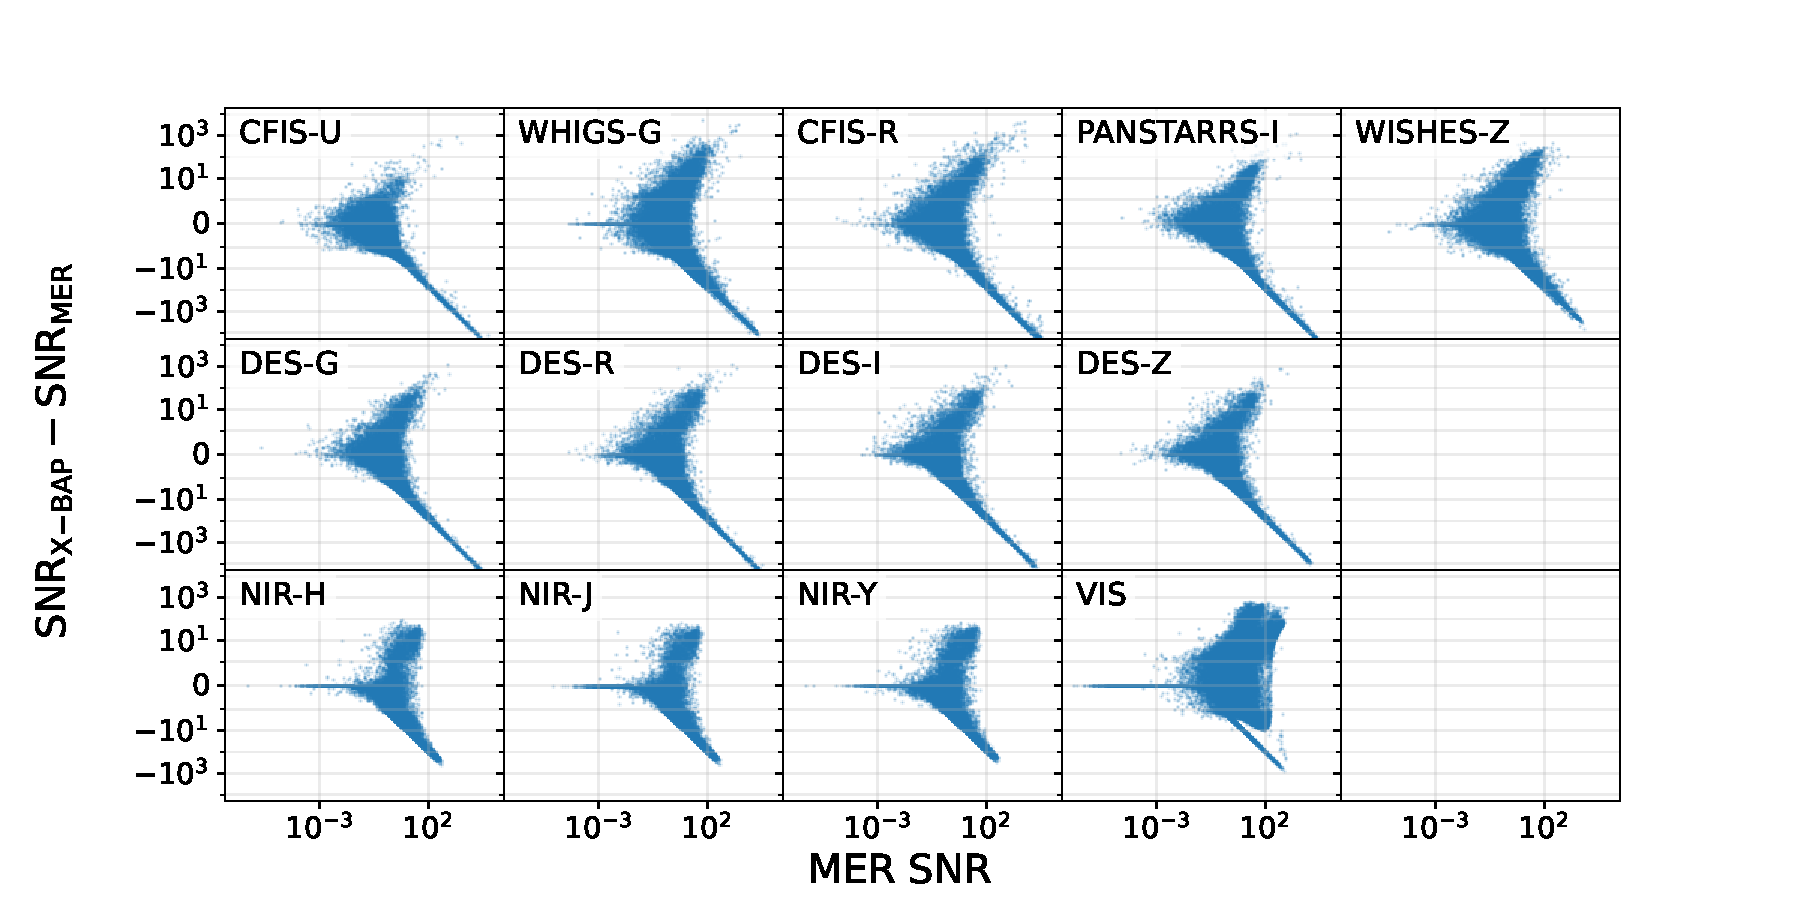
\includegraphics[width=\linewidth]{results/figures/analysis/snr_comparison.pdf}
    \caption{Comparison of \gls{snr} from \gls{x-bap} and the \gls{mer} catalog for all catalog filters. The dashed line denotes equal \gls{snr}. The measurements are from tiles 102022978 (top row), 102158274 (middle row), and 102158274 (bottom row).}
    \label{fig: snr comparison correlated}
\end{figure}
The results in \autoref{fig: snr comparison correlated} show a similar behavior, where the \gls{snr} of the sources, especially towards higher \gls{snr}, is lower for the \gls{x-bap} method compared to the method used to calculate the flux in the \gls{mer} catalogs.
\textbf{INCLUDE MORE STATISTICS FOR THE COMPARISON}


% \subsection{Observation Results: Photometric Redshift}
% parameters explained

% compared redshift statistics derived from pca-phot flux to those derived from MER

% \begin{figure}[H]
%     \centering
%     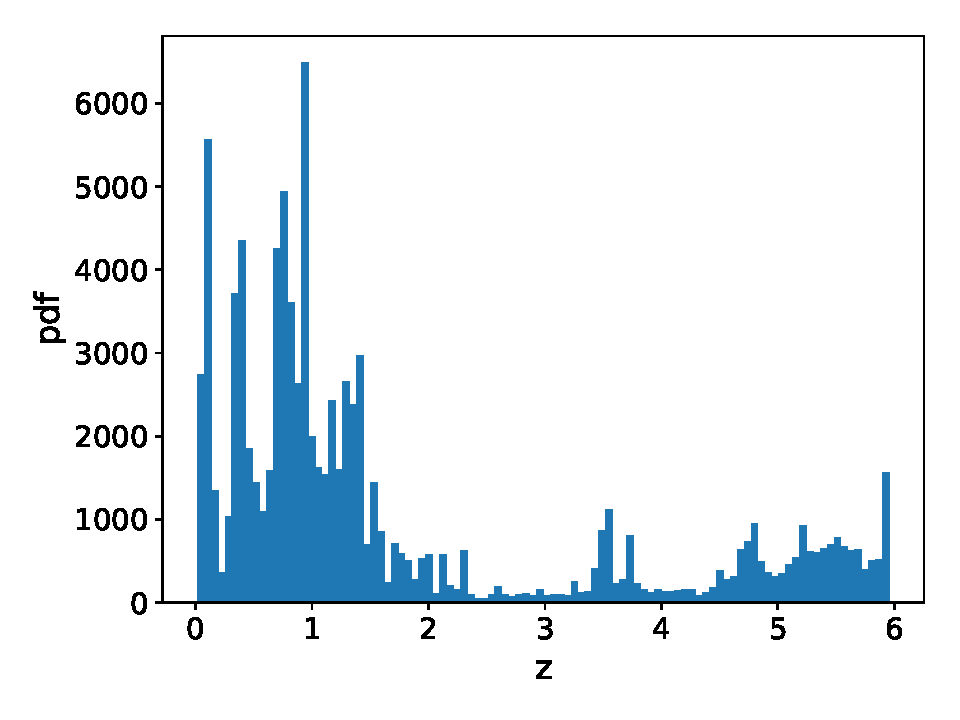
\includegraphics[width=0.5\linewidth]{results/figures/analysis/z_distribution.pdf}
%     \caption{Distribution of photometric redshifts in the field 53.00 -28.00.}
%     \label{fig: z distribution}
% \end{figure}

% spectroscopic redshift?


% \citep{brammer_eazy_2008}
\subsection{Classification}


Following a similar procedure as \cite{euclid_collaboration_euclid_2026}, the colors of the objects in the \gls{mer}is tiles are used to classify the objects. In addition to the colors, the fractional difference between the aperture fluxes for different weight sizes is used to classify the sources as point-like or extended. The goal is to classify the sources into one of three categories: stars, galaxies, and \glspl{qso}.

\subsubsection{Splitting Sources}\label{subsec: Splitting Sources}


Here, \gls{umap} \citep{mcinnes_umap_2018} is used to reduce the dimensionality of all the color information of the sources. This is done for the tiles in the \gls{edfn} and for the tiles in \gls{edff} and \gls{edfs}.

\begin{figure}[H]
    \centering

    \begin{subfigure}{0.45\textwidth}
        \centering
        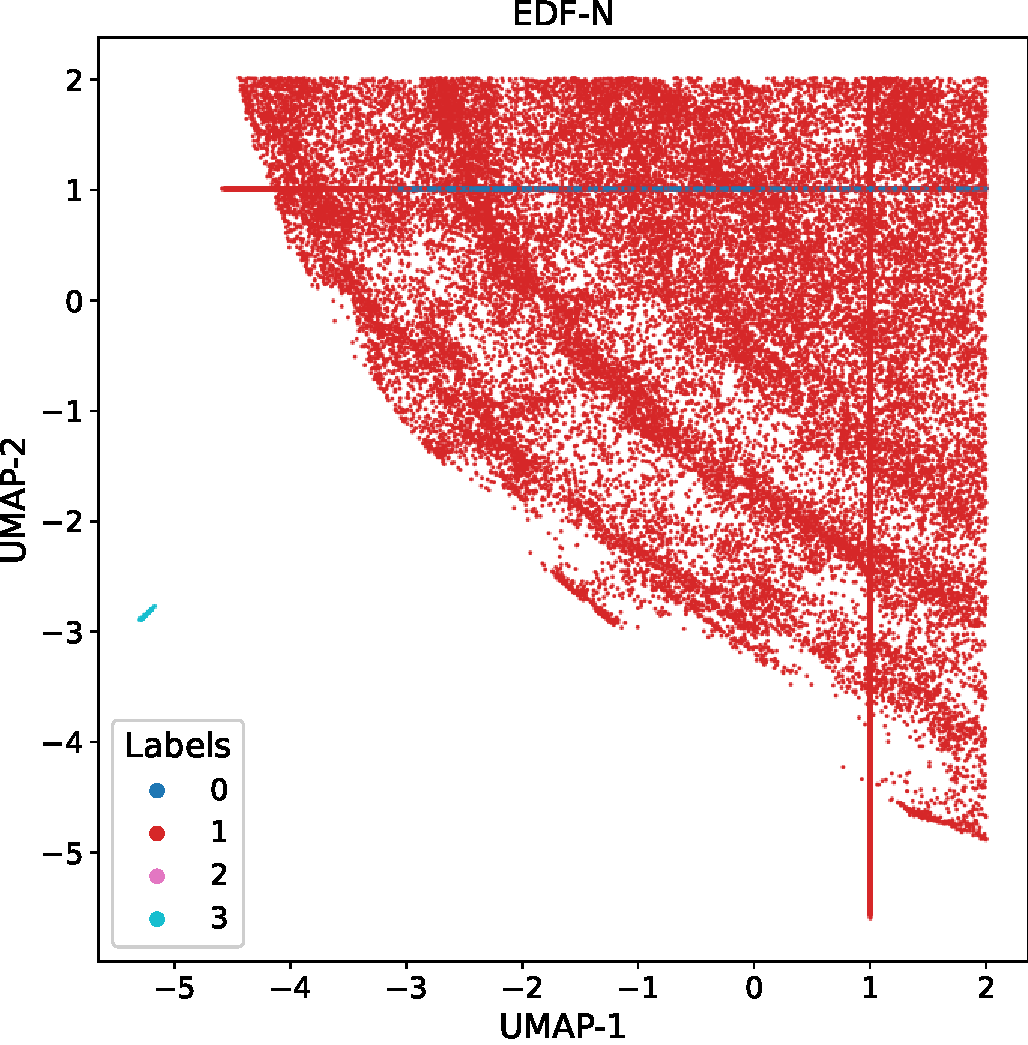
\includegraphics[width=\linewidth]{results/figures/analysis/UMAP_splitting_north.pdf}
        % \caption{First image}
        % \label{fig: umap splitting north}
    \end{subfigure}
    \hfill
    \begin{subfigure}{0.45\textwidth}
        \centering
        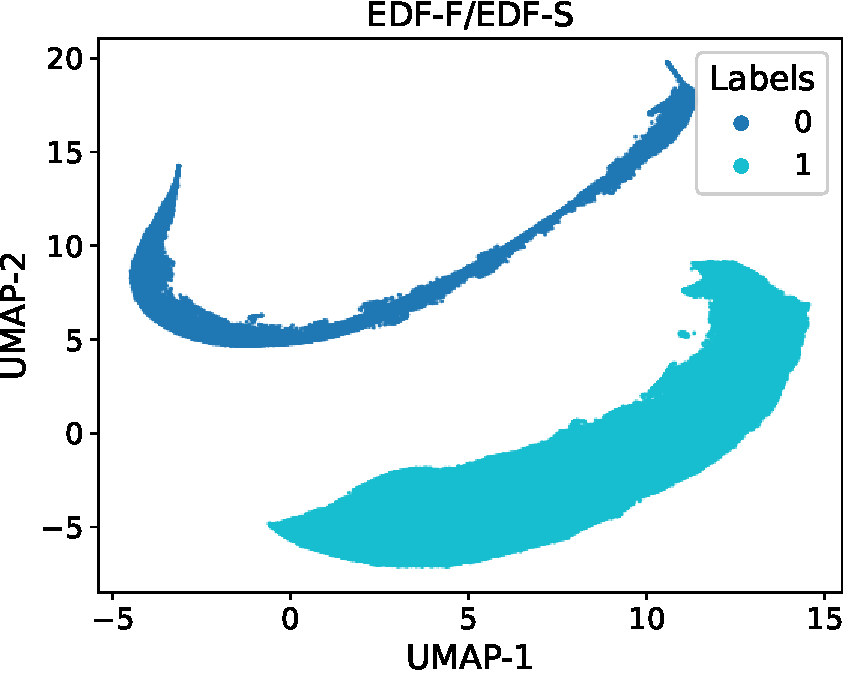
\includegraphics[width=\linewidth]{results/figures/analysis/UMAP_splitting_south.pdf}
        % \caption{Second image}
        % \label{fig: umap splitting south}
    \end{subfigure}
    
    \caption{\gls{umap} dimension reduction of the colors for the objects in the fields \gls{edfn} (left), and \gls{edff}/\gls{edfs} (right). Both show two large clusters of objects which are labeled.}
    \label{fig: umap splitting}
\end{figure}
Using \gls{umap}, 2 large clusters of objects are visible (\autoref{fig: umap splitting}). The structure of the clusters is similar between the 2 fields. The points with label 1 are more shaped as a blob, whereas the points with label0 form a longer string. However, there is no information on which type of object corresponds to these clusters. For this, the colors of the clusters are plotted to show which type of object corresponds to which label.

\begin{figure}[H]
    \centering

    \begin{subfigure}{0.45\textwidth}
        \centering
        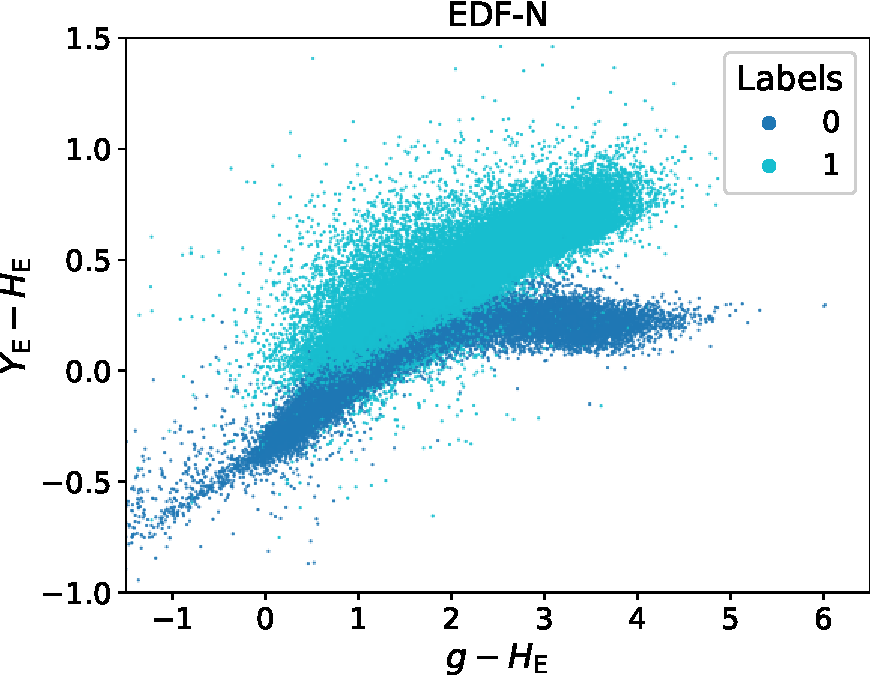
\includegraphics[width=\linewidth]{results/figures/analysis/color_color_splitting_north.pdf}
        % \caption{First image}
        % \label{fig: color color splitting north}
    \end{subfigure}
    \hfill
    \begin{subfigure}{0.45\textwidth}
        \centering
        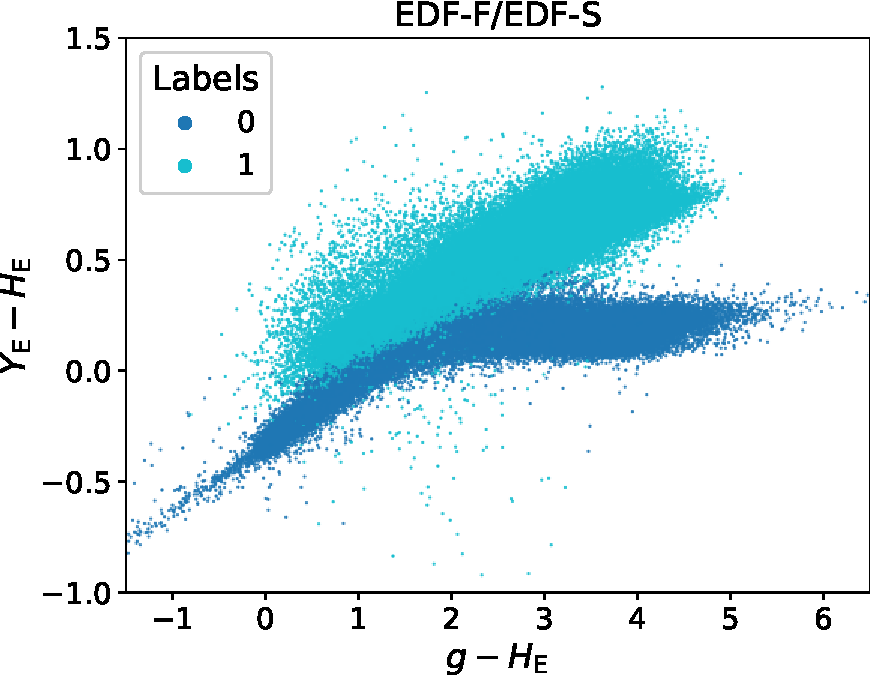
\includegraphics[width=\linewidth]{results/figures/analysis/color_color_splitting_south.pdf}
        % \caption{Second image}
        % \label{fig: color color splitting south}
    \end{subfigure}
    
    \caption{Color-color diagram of objects in the fields \gls{edfn} (left), and \gls{edff}/\gls{edfs} (right). The objects are split based on the labels in \autoref{fig: umap splitting}.}
    \label{fig: color color splitting}
\end{figure}
\autoref{fig: color color splitting} shows that sources labeled 1 have redder Y-H colors at given g-H colors than those labeled 0. Furthermore, the sources labeled 0 are at the loci expected for stars. Therefore, the objects with label 0 are tagged as star-like objects and the objects with label 1 are tagged as galaxy-like objects.

\subsubsection{Star-like Objects}
The star-like objects (labeled 0 in \autoref{subsec: Splitting Sources}) are split into smaller groups once more, using the colors in the same way as for the splitting of the objects into star-like and galaxy-like, but information on the difference in between the fluxes measured using the different weight sizes is also provided into the model, which gives information about the size of the object in the images.  

\begin{figure}[H]
    \centering
    
    \begin{subfigure}{0.45\textwidth}
        \centering
        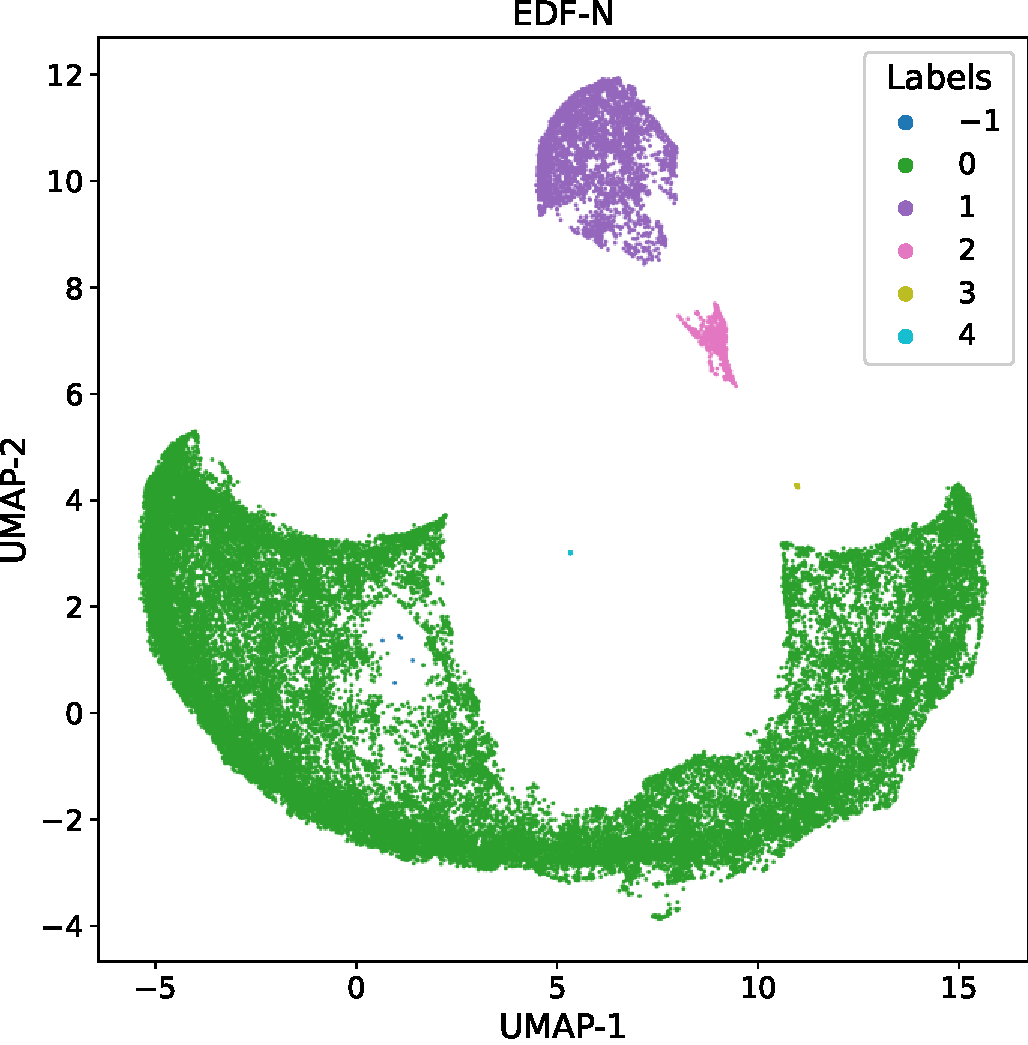
\includegraphics[width=\linewidth]{results/figures/analysis/UMAP_star_north.pdf}
        % \caption{First image}
        % \label{fig: umap star north}
    \end{subfigure}
    \hfill
    \begin{subfigure}{0.45\textwidth}
        \centering
        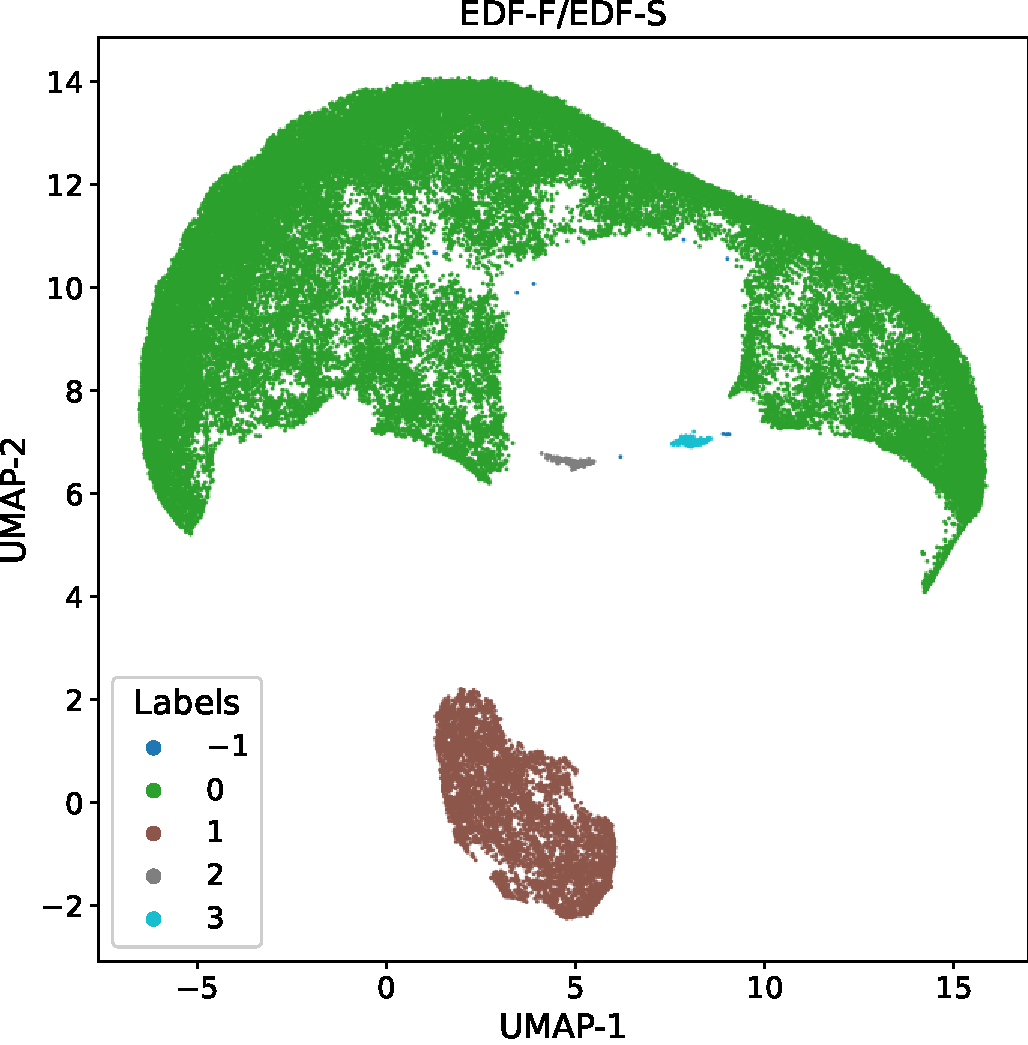
\includegraphics[width=\linewidth]{results/figures/analysis/UMAP_star_south.pdf}
        % \caption{Second image}
        % \label{fig: umap star south}
    \end{subfigure}
    
    \caption{\gls{umap} dimension reduction of the colors and the fractional difference in the flux between different weight sizes for the objects in the fields \gls{edfn} (left), and \gls{edff}/\gls{edfs} (right). }
    \label{fig: umap star}
\end{figure}
The structure of the sources after the dimension reduction in both \gls{edfn} and \gls{edff}/\gls{edfs} is very similar. There is a large fraction of the objects that form a semi-circular structure with a hole in it. Besides that large collection of sources, there is a smaller offshoot of sources that form, in the case of \gls{edfn}, two clusters, and for  \gls{edff}/\gls{edfs} a single cluster.



\begin{figure}[H]
    \centering
    
    \begin{subfigure}{0.45\textwidth}
        \centering
        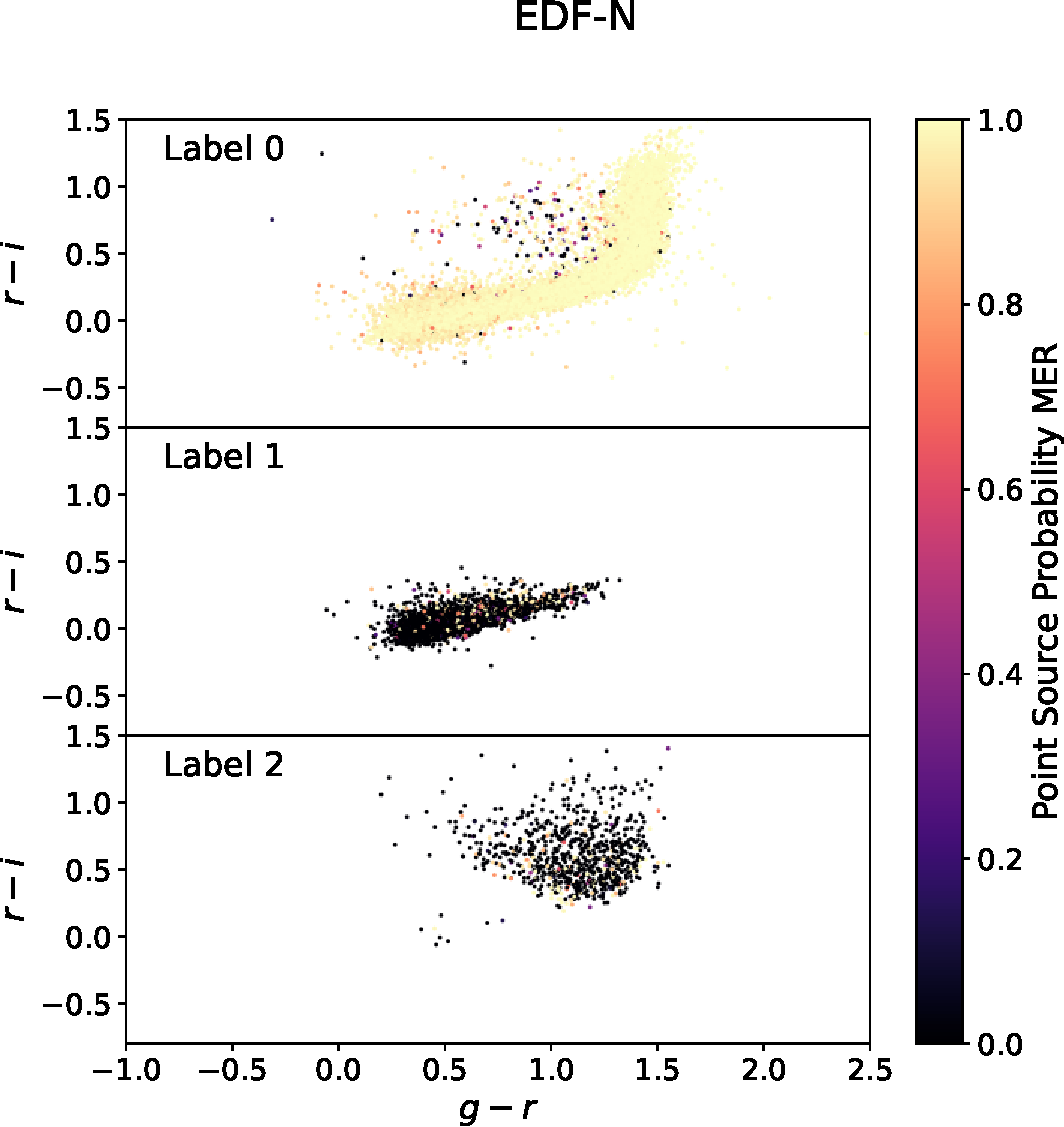
\includegraphics[width=\linewidth]{results/figures/analysis/color_color_star_north.pdf}
        % \caption{First image}
        % \label{fig: color color star north}
    \end{subfigure}
    \hfill
    \begin{subfigure}{0.45\textwidth}
        \centering
        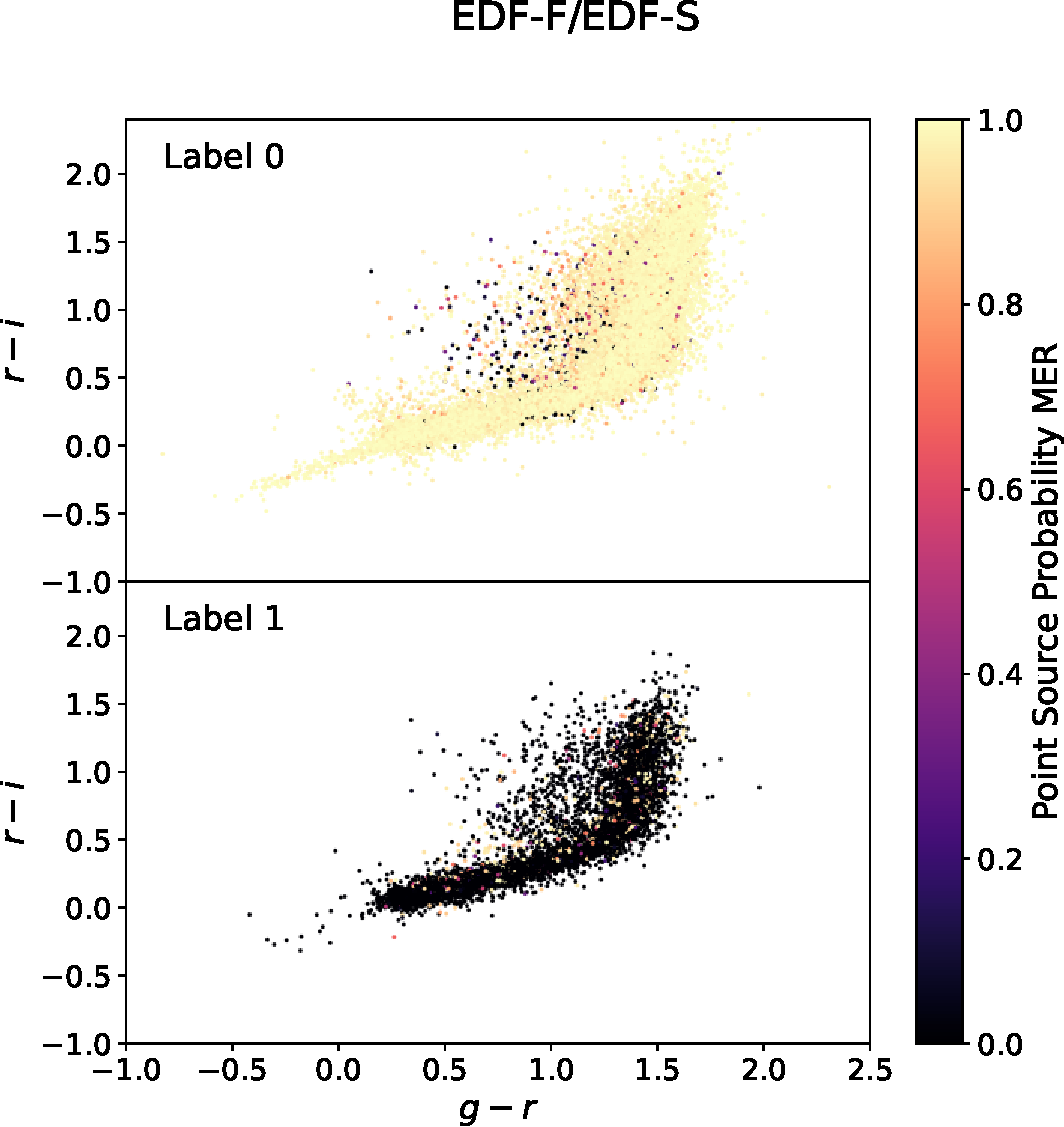
\includegraphics[width=\linewidth]{results/figures/analysis/color_color_star_south.pdf}
        % \caption{Second image}
        % \label{fig: color color star south}
    \end{subfigure}
    
    \caption{Color-color diagram of objects in the fields \gls{edfn} (left), and \gls{edff}/\gls{edfs} (right). The objects are split based on the labels in \autoref{fig: umap splitting}.}
    \label{fig: color color star}
\end{figure}

% \begin{figure}[H]
%     \centering

%     % First row
%     \begin{subfigure}{0.45\textwidth}
%         \centering
%         
\includegraphics[width=\linewidth]{report/layout/figures/leidenuniv_logos/Observatory.pdf}
%         \caption{Image 1}
%         \label{fig:img1}
%     \end{subfigure}
%     \hfill
%     \begin{subfigure}{0.45\textwidth}
%         \centering
%         
\includegraphics[width=\linewidth]{report/layout/figures/leidenuniv_logos/Observatory.pdf}
%         \caption{Image 2}
%         \label{fig:img2}
%     \end{subfigure}

%     \vspace{0.5cm}

%     % Second row
%     \begin{subfigure}{0.45\textwidth}
%         \centering
%         
\includegraphics[width=\linewidth]{report/layout/figures/leidenuniv_logos/Observatory.pdf}
%         \caption{Image 3}
%         \label{fig:img3}
%     \end{subfigure}
%     \hfill
%     \begin{subfigure}{0.45\textwidth}
%         \centering
%         
\includegraphics[width=\linewidth]{report/layout/figures/leidenuniv_logos/Observatory.pdf}
%         \caption{Image 4}
%         \label{fig:img4}
%     \end{subfigure}

%     \caption{IMAGES OF THE OBJECT IN THIS CLASSIFICATION, BOTH LABELS AND BOTH NORTH AND SOUTH}
%     \label{fig:grid}
% \end{figure}


About xx\% of the objects that have colors similar to stars found using the \gls{umap} clustering have a low point-source-probability following the \gls{mer} catalog. Visually examining these objects shows (\autoref{fig: Extended stars}) that they are close to bright stars. As the weight function is bigger than the biggest \gls{psf} of the filters considered, the close star becomes a considerable portion of the flux measured. So the flux is dominated by the star that is close to the object, resulting in star-like colors. 

\begin{figure}[H]
    \centering
    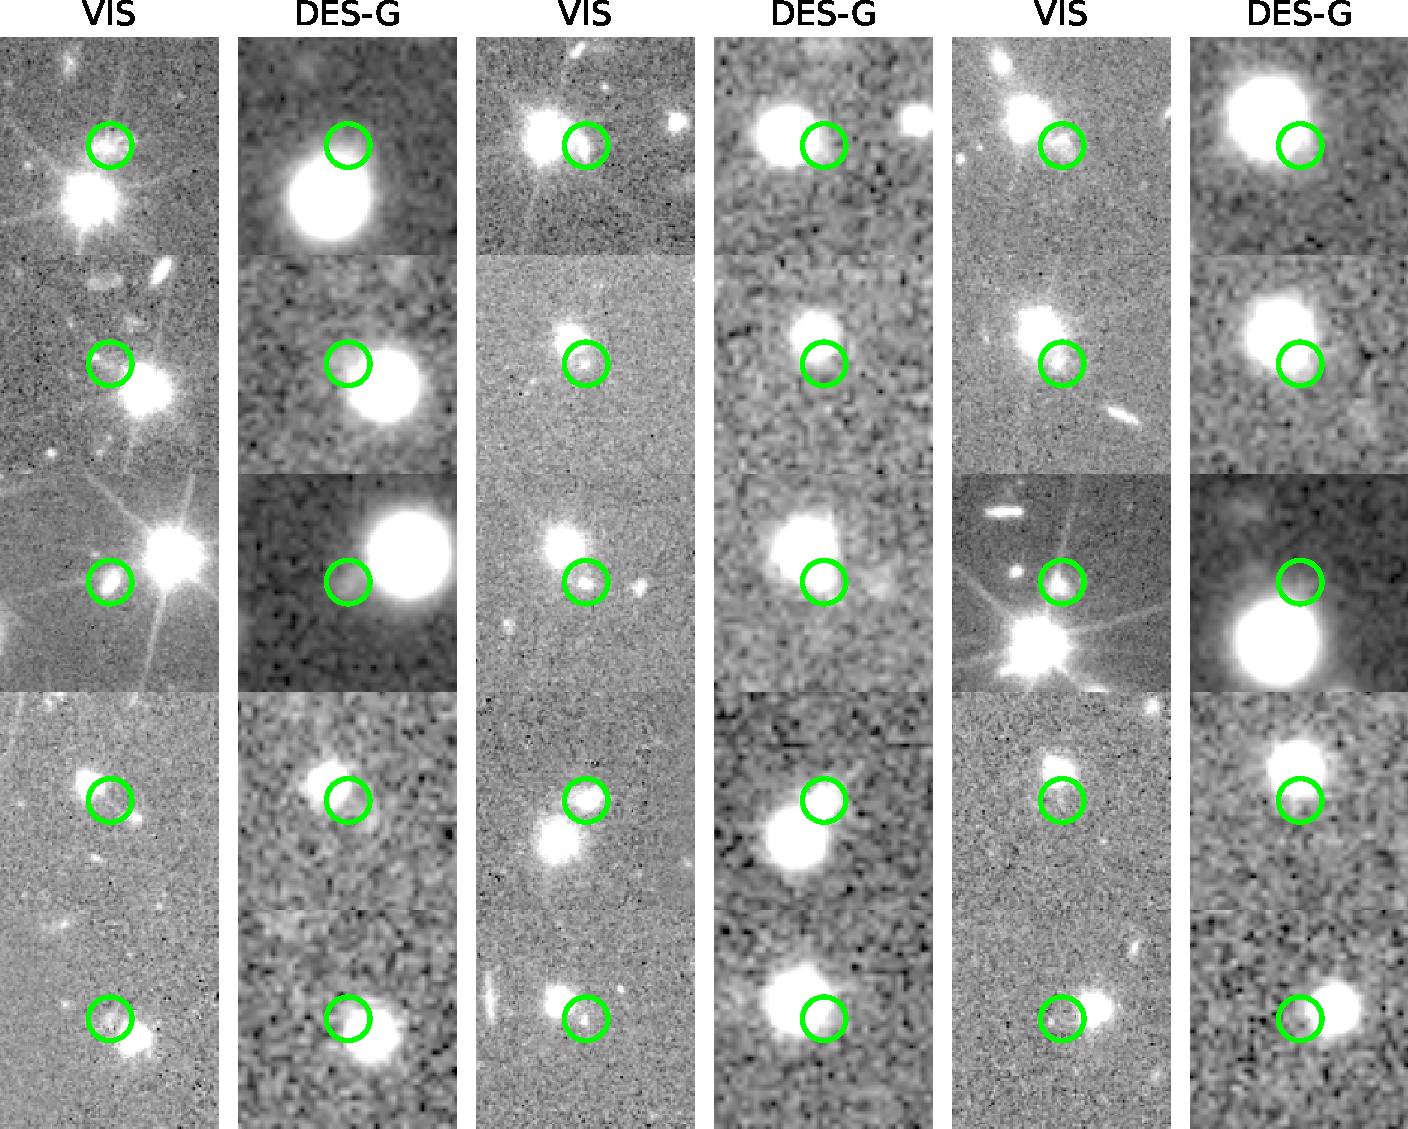
\includegraphics[width=0.8\linewidth]{results/figures/observation/blended_object.pdf}
    \caption{Sources in tile 102021503 (\gls{edff}/\gls{edfs}) that have a label 1 according to the \gls{umap} dimension reduction shown in \autoref{fig: umap star}. The centers of the objects are highlighted by a lime circle. Most of the objects shown are clearly visible in the \gls{vis}, but are blended in the \gls{des}-G.}
    \label{fig: Extended stars}
\end{figure}
\cite{euclid_collaboration_euclid_2026} have also classified the objects based on the fluxes; a comparison between their results and the results of the clustering is shown in \autoref{tab: star-like comparison}.

\begin{table}[H]
\centering
\begin{tabular}{lcccccccc}
\toprule
Set & Uncl. & Star & Galaxy & S+G & \gls{qso} & S+Q & G+Q & S+G+Q \\
\midrule
\multicolumn{9}{l}{\textbf{\gls{edfn}}} \\
label 0 & \input{results/tables/star/north/0.txt} \\
label 1 & \input{results/tables/star/north/1.txt} \\
label 2 & \input{results/tables/star/north/2.txt} \\
\addlinespace
\midrule
\multicolumn{9}{l}{\textbf{\gls{edff}/\gls{edfs}}} \\
label 0 & \input{results/tables/star/south/0.txt} \\
label 1 & \input{results/tables/star/south/1.txt} \\
\bottomrule
\end{tabular}
\caption{Classification of the objects with labels according to the \gls{phz} catalog. The objects are either flagged as unclassified, or as star, galaxy, or \gls{qso} or a combination of the three.}
\label{tab: star-like comparison}
\end{table}
The sources that have label 0 are largely classified as stars by \cite{euclid_collaboration_euclid_2026}, which is also what is expected from the point-source-probability in the \gls{mer} catalog. 


\subsubsection{Galaxy-like Objects}

After the splitting of the sources based on the colors derived from the  1\gls{fwhm} flux, the colors of both 0.5\gls{fwhm} and 2\gls{fwhm} are used to split the sources further. As stated in \autoref{WHERE EXPLAINED HOW POINTSOURCES DETECTED}, the colors derived using different weight sizes should give information about the physical size of the source in the image and thus can help to differentiate the \glspl{qso} from the galaxies. As before, UMAP is used to reduce the dimensionality of the colors and the relative difference in the flux of the different weight sizes.
\begin{figure}[H]
    \centering

    \begin{subfigure}{0.45\textwidth}
        \centering
        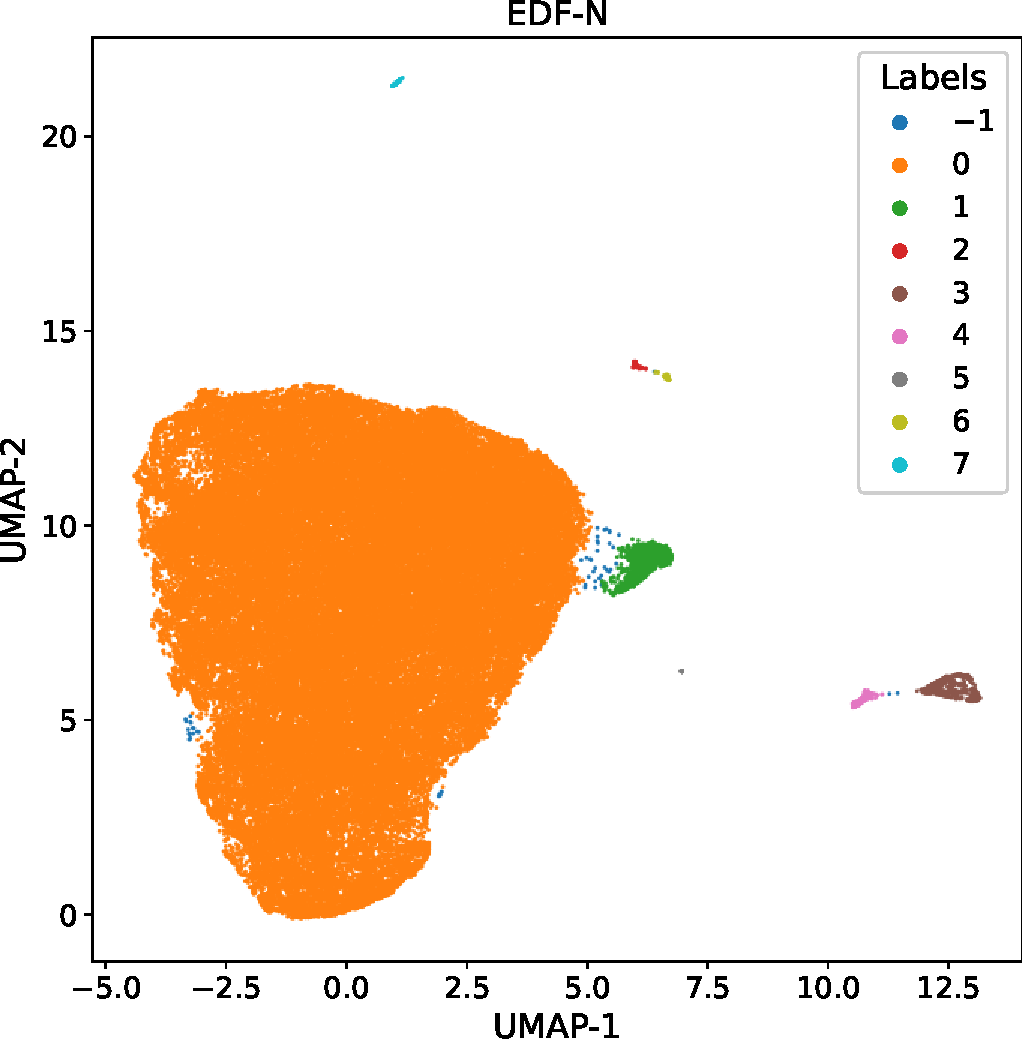
\includegraphics[width=\linewidth]{results/figures/analysis/UMAP_galaxy_north.pdf}
        % \caption{First image}
        % \label{fig: umap galaxy north}
    \end{subfigure}
    \hfill
    \begin{subfigure}{0.45\textwidth}
        \centering
        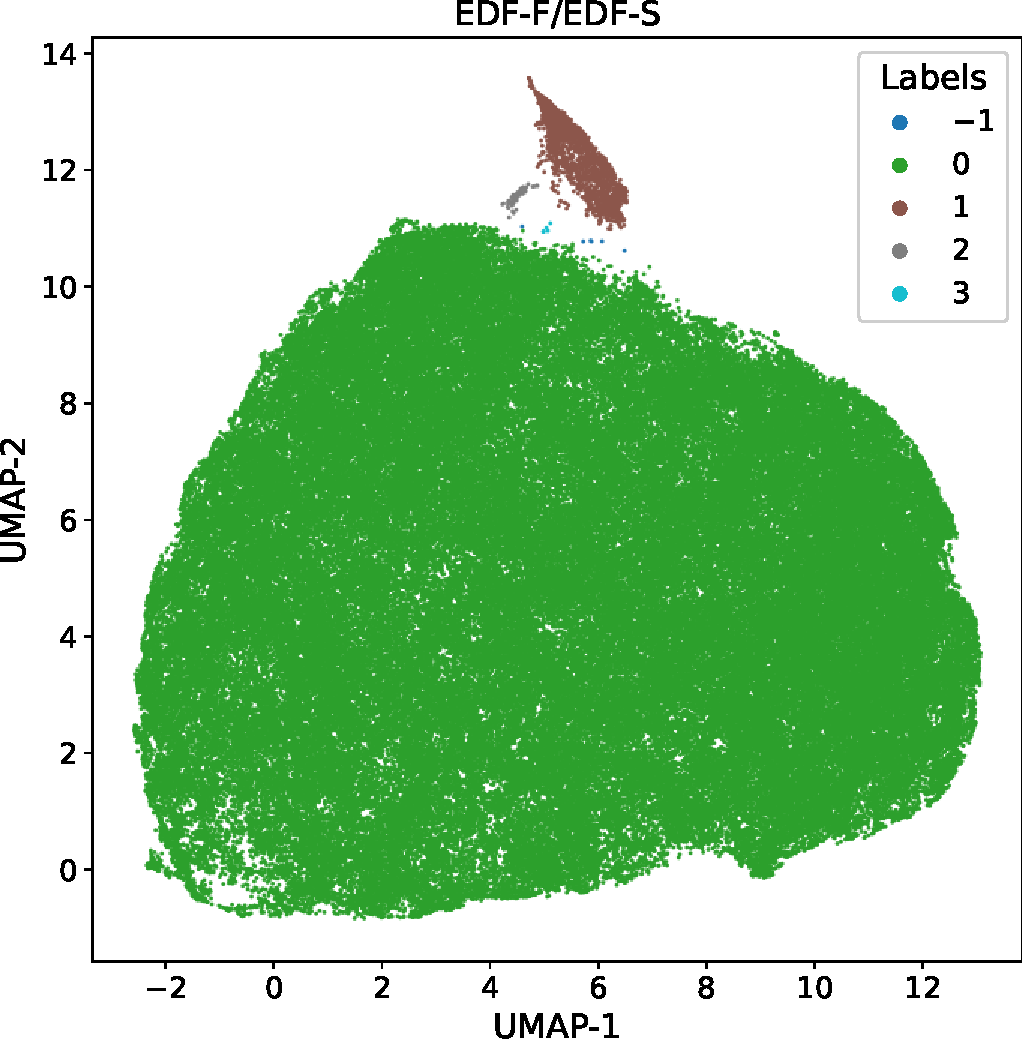
\includegraphics[width=\linewidth]{results/figures/analysis/UMAP_galaxy_south.pdf}
        % \caption{Second image}
        % \label{fig: umap galaxy south}
    \end{subfigure}
    
    \caption{\gls{umap} dimension reduction of the colors and the fractional difference in the flux between different weight sizes for the objects in the fields \gls{edfn} (left), and \gls{edff}/\gls{edfs} (right). }
    \label{fig: umap galaxy}
\end{figure}

The \gls{umap} dimension reduction shows a similar structure for both the \gls{edfn} and \gls{edff}/\gls{edfs}, where there is one large cluster of objects and then a smaller cluster close to it. Furthermore, in the field \gls{edfn} there are several additional smaller clusters. Looking at which tiles the objects originate from shows that the sources in these smaller clusters are only present in a small number of tiles. This indicates that there might be some error in the measurements or calibration for these tiles, resulting in the deviating behavior.

\begin{figure}[H]
    \centering
    
    \begin{subfigure}{0.45\textwidth}
        \centering
        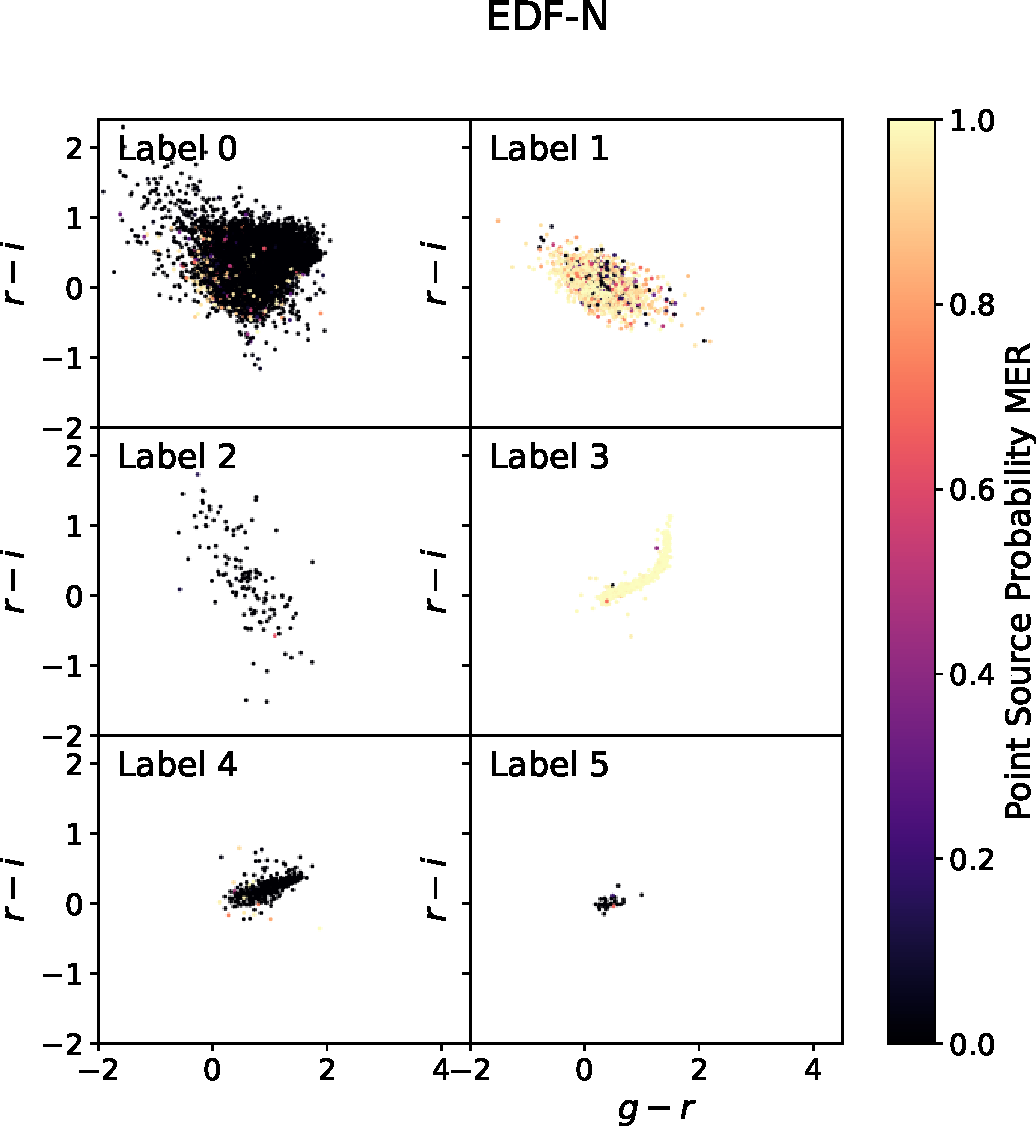
\includegraphics[width=\linewidth]{results/figures/analysis/color_color_galaxy_north.pdf}
        % \caption{First image}
        % \label{fig: color color galaxy north}
    \end{subfigure}
    \hfill
    \begin{subfigure}{0.45\textwidth}
        \centering
        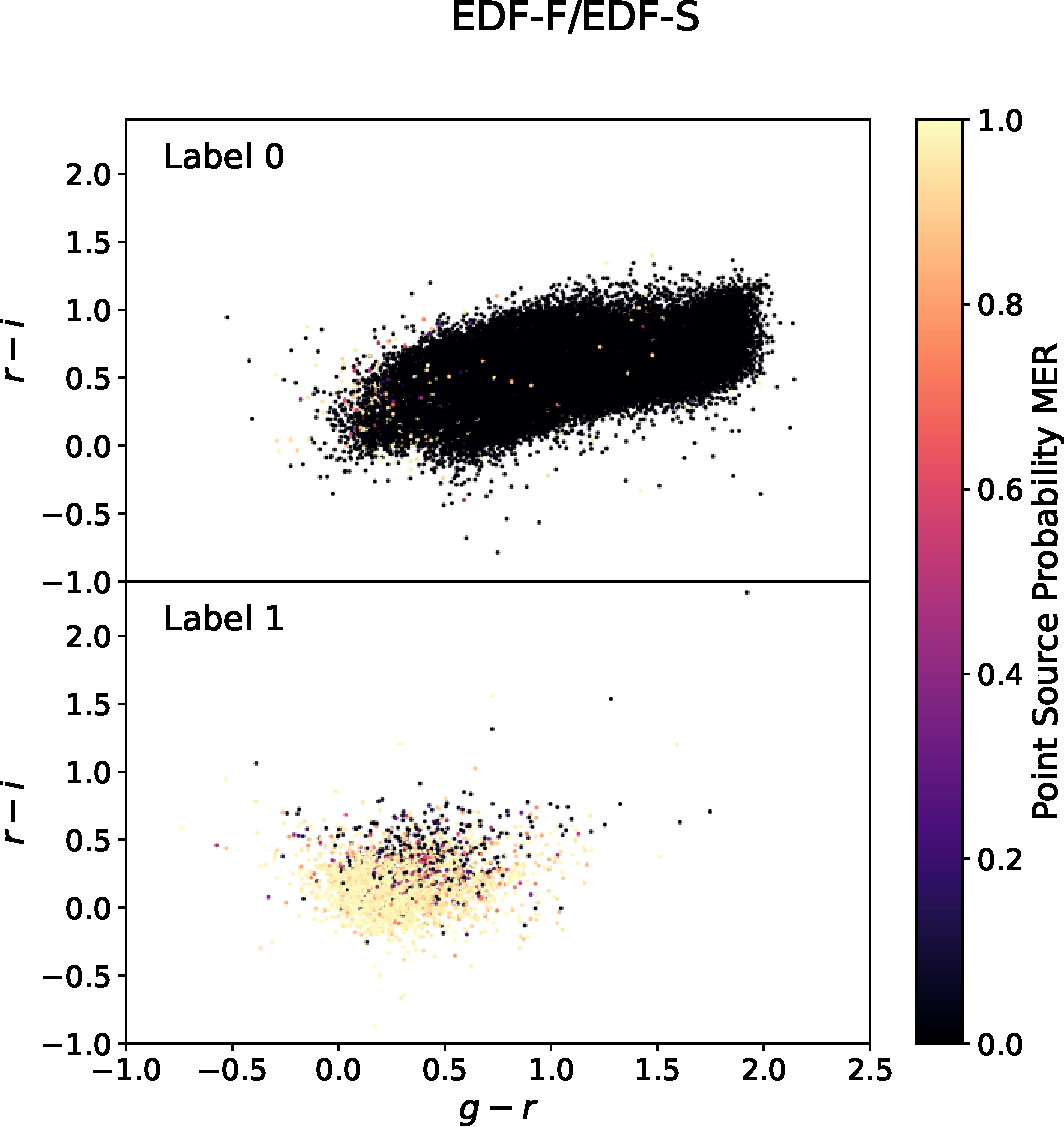
\includegraphics[width=\linewidth]{results/figures/analysis/color_color_galaxy_south.pdf}
        % \caption{Second image}
        % \label{fig: color color galaxy south}
    \end{subfigure}
    
    \caption{Color-color diagram of objects in the fields \gls{edfn} (left), and \gls{edff}/\gls{edfs} (right). The objects are split based on the labels in \autoref{fig: umap splitting}.}
    \label{fig: color color galaxy}
\end{figure}

This shows that for both \gls{edfn} and \gls{edff}/\gls{edfs} there are sources that have a high point-source-probability. Notably, \gls{edfn} has a third group with different behavior that has a similar structure as star-like sources. However, this group only contains objects that are only from 3 tiles. This group will be discussed in \autoref{subsec: Tiles with Different Colors}. A comparison with the labels found here and the classifications following the \gls{phz} catalog is shown in \autoref{tab: galaxy}.

\begin{table}[H]
\centering
\begin{tabular}{lcccccccc}
\toprule
Set & Uncl. & Star & Galaxy & S+G & \gls{qso} & S+Q & G+Q & S+G+Q \\
\midrule
\multicolumn{9}{l}{\textbf{\gls{edfn}}} \\
label 0 & \input{results/tables/galaxy/north/0.txt} \\
label 1 & \input{results/tables/galaxy/north/1.txt} \\
label 2 & \input{results/tables/galaxy/north/2.txt} \\
label 3 & \input{results/tables/galaxy/north/3.txt} \\
label 4 & \input{results/tables/galaxy/north/4.txt} \\
label 5 & \input{results/tables/galaxy/north/5.txt} \\
\addlinespace
\midrule
\multicolumn{9}{l}{\textbf{\gls{edff}/\gls{edfs}}} \\
label 0 & \input{results/tables/galaxy/south/0.txt} \\
label 1 & \input{results/tables/galaxy/south/1.txt} \\
\bottomrule
\end{tabular}
\caption{Classification of the objects with labels according to the \gls{phz} catalog. The objects are either flagged as unclassified, or as star, galaxy, or \gls{qso} or a combination of the three.}
\label{tab: galaxy}
\end{table}
The label 0 sources are expected to be mostly galaxies, which is also the result of the comparison with the results from the \gls{phz} catalog. The label 1 sources are expected to be the \glspl{qso}. In the case of \gls{edfn}, \~10.5\% of the sources are flagged as \gls{qso} in the \gls{phz} catalog. For \gls{edff}/\gls{edfs} almost none of the sources are flagged as \gls{qso} by the \gls{phz} catalog. This is most likely due to the missing $u$ band in these fields, which gives more information about bluer light than the other filters. This missing information makes it harder to flag the sources as \gls{qso}.  

% \begin{figure}[H]
%     \centering

%     % First row
%     \begin{subfigure}{0.45\textwidth}
%         \centering
%         
\includegraphics[width=\linewidth]{report/layout/figures/leidenuniv_logos/Observatory.pdf}
%         \caption{Image 1}
%         \label{fig:img1}
%     \end{subfigure}
%     \hfill
%     \begin{subfigure}{0.45\textwidth}
%         \centering
%         
\includegraphics[width=\linewidth]{report/layout/figures/leidenuniv_logos/Observatory.pdf}
%         \caption{Image 2}
%         \label{fig:img2}
%     \end{subfigure}

%     \vspace{0.5cm}

%     % Second row
%     \begin{subfigure}{0.45\textwidth}
%         \centering
%         
\includegraphics[width=\linewidth]{report/layout/figures/leidenuniv_logos/Observatory.pdf}
%         \caption{Image 3}
%         \label{fig:img3}
%     \end{subfigure}
%     \hfill
%     \begin{subfigure}{0.45\textwidth}
%         \centering
%         
\includegraphics[width=\linewidth]{report/layout/figures/leidenuniv_logos/Observatory.pdf}
%         \caption{Image 4}
%         \label{fig:img4}
%     \end{subfigure}

%     \caption{IMAGES OF THE OBJECT IN THIS CLASSIFICATION, BOTH LABELS AND BOTH NORTH AND SOUTH}
%     \label{fig:grid}
% \end{figure}

\subsubsection{Tiles with Deviating Colors}\label{subsec: Tiles with Different Colors}
Three tiles show a different color from the other tiles in the galaxy-like coloring of the objects: 102021578, 102021579, and 102021579. 

\begin{figure}[H]
    \centering
    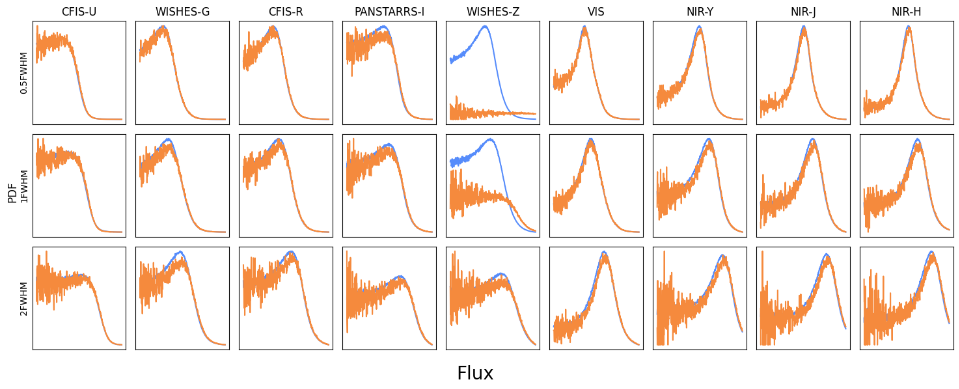
\includegraphics[width=0.9\linewidth]{results/figures/analysis/flux_cmparison.png}
    \caption{Distribution of the measured aperture fluxes on a logarithmic scale. The yellow lines are the distribution of fluxes in the tiles 102021578, 102021579, and 102021579. The blue lines are the distribution of fluxes in all the other tiles. For each band, both align well except for in the case of $z$ where they strongly deviate, especially for smaller aperture sizes.}
    \label{fig: }
\end{figure}

Here, the distribution of the measured fluxes in the WISHES-Z band for these tiles differs from that of the other tiles. 
\textbf{REASON WHY DO THESE TILES DEVIATE?}